\section{Performance Evaluation}\label{sec:perf}

The PBBS benchmark consists of three data sets. Each of these consists of
$10^8$ points drawn from different distributions. Even though all data sets
are $1.6$ GB in size, the algorithm behaves very differently on them.

\tkcomment{TODO: do this properly. Also, do Qhull, CGAL give indices
           or points? If they give indices too, why?}
As a baseline we have considered Qhull, the algorithms of CGAL,
and the implementation of PBBS. Some preliminary testing shows that the
implementation of PBBS is the fastest by a large margin. In
Table~\ref{table:reference} are the runtimes for a disk of $10^7$ points.

\begin{table}[ht]
    \caption{Runtime in seconds for a disk of $10^7$ points}
    \label{table:reference}
    \begin{tabular}{c | c }
     Implementation & Runtime \\ 
     \hline \\
     PBBS & 0.31 \\  
     CGAL Quickhull & 0.61 \\
     CGAL Akl-Toussaint & 0.60 \\
     CGAL Bykat & 0.73 \\
     CGAL Eddy & 0.98 \\
     CGAL Graham & 1.3 \\
     CGAL Jarvis & 208 \\
     Qhull & TODO, but slow \\
    \end{tabular}
\end{table}

We use GCC 14.1.1. All experiments are run 20 times. The standard deviation is 
less than $2.5\%$ in all cases, so we only report the means.

\subsection{Evaluation Platforms}

We evaluate our implementation on two machines. The first, \textit{cn125}
has powerful vector instructions, a modest amount of cores and memory, and a 
simple memory architecture. 

The second, \textit{cn132}, has less powerful vector instructions and needs
to emulate the compress of ... It has two CPUs which gives it more cores
and memory bandwidth. Memory is local to one of the two CPUs, so we need
to make sure allocations are equally distributed between the two. We have
done this by running the programs under \texttt{numactl --interleaved all}.

We summarize the systems in Table~\ref{tab:system}. There can be a significant
gap between the bandwidth the RAM is capable off, and what is achievable in
practice. The STREAM benchmark \cite{} is a collection of simple functions
that can be used to measure what bandwidths can be achieved in practice.

\begin{table}
    \caption{Theoretical and practical capabilities of test systems. All four
             STREAM benchmarks obtained the same bandwidth.}
    \label{tab:system}
    \begin{tabular}{c|c|c}
                                   & cn132 & cn125          \\
        \hline                                              
        CPU                        & Epyc 7313 $(\times 2)$ 
                                           & Xeon E-2378    \\
        Vector extension           & avx2  & avx512         \\
        Frequency (GHz)            & 3.7   & 2.6            \\
        Peak compute rate (Gflops) & 1894  & 346            \\
        Theoretic bandwidth (GB/s) & 204.8 & 51.2           \\ 
        STREAM (GB/s)              & 140   & 38             \\ 
    \end{tabular}
\end{table}

\subsection{The Data Sets}\label{subsec:datasets}

There is a large difference between runtime of Quickhull on the different 
datasets.
To gain insight, we make a rough estimation of the amount of work required.
\tkcomment{I suppose we can measure this, but the work per pass over the
data may also be interesting.}

\subsubsection{Kuzmin}

Whereas Circle and Disk are symmetric, Kuzmin is very much the opposite
as illustrated in Figure~\ref{fig:kuzmin}.
The first two partitions end up with almost all points either in $S_1$ or
in $S_2$, and on the subsequent partition almost all points are discarded.
The convex hull has only $4$ points.

\begin{figure}[ht]
    \includegraphics[width=0.3\columnwidth]{./figures/rust-kuzmin.png}
    \caption{The Kuzmin dataset of $10^8$ points. The first partition only
             moves $r_1$. The second partition eliminates all remaining points.}
    \label{fig:kuzmin}
\end{figure}

\subsubsection{Circle}

A circle is convex, so all points are on the hull. As a circle is symmetric,
each recursive call of FindHull will identify an element on the hull, and
then recurse on two subsets $S_1$ and $S_2$ differing at most one in size.
That means we have $2^d$ calls at recursion depth $d$ until we hit the point 
where either $|S_1| = 1$ and $|S_2| = 0$ or vice-versa. 
As each recursive call eliminates one point, there are
$10^8 - \sum_{i = 0}^{d - 1} 2^i = 10^8 - 2^{d}$ points left at recursion 
depth $d$. For $10^8$ points, we have a recursion depth of 
$\lceil \log_{2}(10^8) \rceil = 26$.

\textbf{A note on accuracy: }as the circle has effectively area $0$, the 
points are much closer together than in the other data sets.
This causes some accuracy difficulties. Already for 100K points, 
both BlockQuickhull and PBBS do not report all points as being in the hull. Both 
implementations find the same points up to 10M points, after which they disagree
on $20$ points. These are points $u$ for which $\text{orient}(p, u, r_1) > 0$
and $\text{orient}(r_2, u, q) > 0$, so this is because of our choice to put
these in $S_1$. 

\subsubsection{Disk}

The first recursion will identify $p$, $r_1$, $q$, $r_2$ as lying on the
convex hull, and partition the points into those above and below $pq$.
Then the second partition will eliminate region V of 
Figure~\ref{fig:disk_level2}. This square has area $2$, so it will eliminate
most points: a fraction $\frac{2}{\pi} \approx 0.637$.

\begin{figure}[ht]
    \resizebox{\columnwidth}{!}{%
        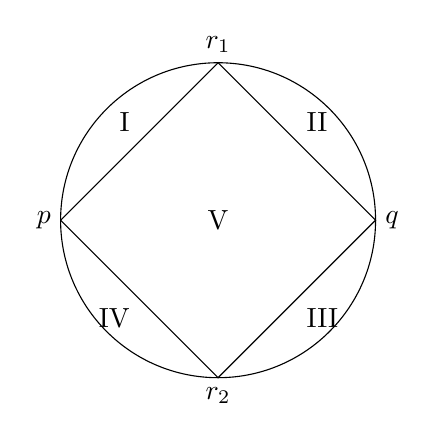
\begin{tikzpicture}
            \draw (0, 0) circle (2);
            \draw (-2, 0) node[left]  {$p$}   -- node[pos=0.5, above left] {I}
                  (0, 2)  node[above] {$r_1$} -- node[pos=0.5, above right] {II}
                  (2, 0)  node[right] {$q$}   -- node[pos=0.5, below right] {III}
                  (0, -2) node[below] {$r_2$} -- node[pos=0.5, below left] {IV}
                  (-2, 0);
                  \node at (0, 0) {V};
        \end{tikzpicture}
    }
    \caption{The Disk data set at recursion level 2. Region V will be 
             eliminated, and the recursion will continue on regions I 
             \textemdash IV.}
    \label{fig:disk_level2}
\end{figure}

After this, the recursion will continue on pie slices of progressively smaller
angle. The proportion of points eliminated is almost constant in this angle.
To see this, we label some points in Figure~\ref{fig:disk_level3+}. 

\begin{figure}[ht]
    \resizebox{\columnwidth}{!}{%
        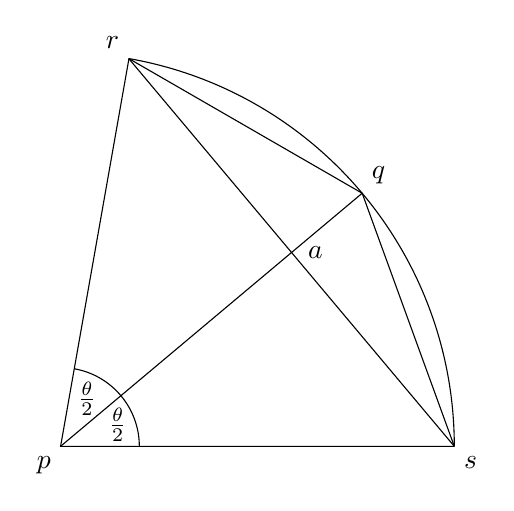
\begin{tikzpicture}
            \foreach \r in {5} {
            \draw (0,0) arc (0:80:\r);
            \draw (-0.8 * \r,0) arc (0:80:0.2 * \r) 
                            node[pos=0.2, left] {$\frac{\theta}{2}$}
                            node[pos=0.88, below] {$\frac{\theta}{2}$};
            \draw (0,0)  node[below right] {$s$} -- ++(0+180:\r) -- 
                                +(80:\r) node[above left] {$r$};
            \draw (-1 * \r,0) node[below left] {$p$} -- 
                  (0.766 * \r - 1 * \r, 0.6428 * \r) node[above right] {$q$};
            \draw (0.173 * \r - 1 * \r, 0.985 * \r) -- (0, 0);
            \draw (0.173 * \r - 1 * \r, 0.985 * \r) -- 
                  (0.766 * \r - 1 * \r, 0.6428 * \r) -- (0, 0);
            \node at (0.413 * \r - 0.766 * \r, 0.766 * 0.6428 * \r) {$a$};
        }
        \end{tikzpicture}
    }
    \caption{Subset of Disk we apply a recursive call of the Quickhull 
             algorithm on. The points are uniformly sampled from the disk
             segment to the right of the line segment $rs$.}
    \label{fig:disk_level3+}
\end{figure}

The elements not yet eliminated lie to the right of $rs$, and in this step,
we eliminate the elements in $\Delta rqs$.

The triangle $\Delta prs$ is isosceles, so $\angle par$ and $\angle pas$
are right angles. That gives us $|pa| = \cos(\theta / 2)$ and 
$|sa| = |ar| = \sin(\theta / 2)$. So $\Delta psr$ has area 
$\sin(\theta / 2) \cos(\theta / 2) = \frac{1}{2} \sin(\theta)$. The entire
pie slice has area $\frac{\theta}{2 \pi} \cdot \pi = \frac{1}{2} \theta$.
Therefore, the part of the circle above the line $rs$ has area 
$\frac{1}{2}(\theta - \sin(\theta))$.

Since $|aq| = |pq| - |pa| = 1 - \cos(\theta / 2)$, the area of $\Delta rqs$
is $\sin(\theta / 2) (1 - \cos(\theta / 2))$. So the fraction of points we
eliminate is

$$\frac{2\sin(\theta / 2) (1 - \cos(\theta / 2))}{\theta - \sin(\theta)}.$$

We approximate this with a third degree Chebyshev approximation on 
$[0, \frac{\pi}{2}]$, which is

% 1.48202191816423201 * 0.5 - -0.00314946736514754 = 0.744160426447263545
% -0.01207255984434141 - 3 * -0.00007573579005338  = -0.01184535247418127
% 2 * -0.00314946736514754                         = -0.00629893473029508
% 4 * -0.00007573579005338                         = -0.00030294316021352
$$0.744 - 0.012 \theta - 0.0063 \theta^2 - 0.0003 \theta^3. $$

The smaller $\theta$ gets, the closer this will be to $0.744$. Even for the
largest $\theta = \frac{\pi}{2}$, this value is reasonably close: $0.708$. 
So we take $0.74$ as approximation. That means the recursion depth is roughly
$1 + \log_{\frac{1}{1 - 0.74}}((1 - 0.637) \cdot 10^8) \approx 14$.

The convex hull has $1593$ points.

\subsection{Interpreting the Results}

Evaluating the performance of an algorithm and its implementation is difficult.
The runtime alone tells us little about the quality of the implementation, as
it differs between machines. We give a few performance measures that can
be related to the capabilities of the machine.

\subsubsection{Bandwidth}

To measure how good our implementation of Quickhull is, we compute the data 
movement required by Quickhull divided by the runtime. The distance between
this and the peak bandwidth of the machine, gives us an
idea of how far the implementation can be improved.

For all datasets, we need to read $10^8$ elements to find the left-most
and right-most point, and then $10^8$ reads and writes to partition $P$
in the set of points above and below the resulting line-segment. A point
is $16$ bytes, so this amounts to $16 \cdot 10^8 \cdot 3 = 4.8 GB$ of 
data-movement. After that, it depends on the data set. We can compute this 
straightforwardly from the analysis of Subsection~\ref{subsec:datasets}.


\textbf{Kuzmin:} after the initial partition into above and below $pq$ of
Figure~\ref{fig:kuzmin}, we only need one read pass to eliminate the
points in $\Delta pr_2q$. This cumulates in a data movement of

$$4.8 \cdot 10^9 + 16 \cdot 10^8 = 6.4 GB.$$ 

\textbf{Circle:} each pass reads and writes all elements in that recursion
level, so the total data movement is

$$4.8 \cdot 10^9 + 2 \cdot 16 \sum_{d = 2}^{26}(10^8 - 2^d) = 81 GB.$$


\textbf{Disk:} on the first recursion we read all points, and write
$1 - \frac{2}{\pi} \approx 0.363$ of those back. From recursion level 2 onwards,
we read all points that are left, and write only a fraction $0.26$ of those
back, so the total data movement is

$$4.8 \cdot 10^9 + (1 + 0.363) \cdot 16 \cdot 10^8 + $$
$$16 \cdot \sum_{d = 1}^{13} 
\left(0.363 \cdot 10^8 \cdot (0.26^{d - 1} + 0.26^{d})\right) =$$
$$8.0 GB.$$

\subsubsection{Effective Bandwidth}

The data movement in this algorithm is not optimal. Take for example 
Figure~\ref{fig:disk_level2}. We could have identified $p$, $r_1$, $q$, $r_2$
in one pass by also keeping track of top and bottom elements. That means
that to reach that stage, we need two reads on $10^8$ elements,
and a write on 
$\left(1 - \frac{2}{\pi}\right) \cdot 10^8 \approx 3.6 \cdot 10^7$ elements.
That would bring the total data movement down from $9.2$ GB to $5.0$ GB.

So to also take possible algorithmic improvements into account,
we also compute the bandwidth as if we did the theoretical minimum of
data movement: one read of the input, and one write for the output.

\subsubsection{Compute Rate}

Computing the orientation of a point takes $7$ flops, and this function is
evaluated twice every time an element is partitioned. So the total number of
flops required is

$$2 \cdot 7 \cdot 2 \cdot 10^8 = 2.8 \cdot 10^9,$$ 
$$2 \cdot 7 \cdot \sum_{d = 1}^{26} (10^8 - 2^d) = 34 \cdot 10^9,$$
$$2 \cdot 7 \cdot 10^8 \cdot 2 + 7 \sum_{d = 1}^{13} \left(0.363^d \cdot 
10^8 \right)  = 3.6 \cdot 10^9.$$

Every clock cycle, the vector units can do $8$ subtractions, multiplications, 
or fmas. We have these in a $4:1:1$ ratio, and they do $1, 1, 2$
flops. The frequency is $2.6$ GHz, so for our computation the peak performance
per core is

$$2.6 \cdot 8 \cdot \frac{4 \cdot 1 + 1 \cdot 1 + 1 \cdot 2}{4 + 1 + 1} = 24.3 
        \ \text{Gflops}.$$

For the entire CPU, this becomes $194$ Gflops.

\subsection{Analysis}

In contrast to our approach, PBBS does not permute the points, but instead
an array of indices pointing to the subsets. This can make for poor spatial
locality in the access of $P$, especially in deeper recursion levels.
It also inhibits vectorization.

For the Kuzmin, almost all points belong in either $S_1$ or $S_2$, so
this dataset is the exception. Similarly, the branches are easy to predict,
giving BlockQuickhull little advantage over the approach of
PBBS. For this reason, we see in Table~\ref{table:runtime} that the deeper
the recursion, the larger our lead over PBBS becomes. 

Kuzmin has to get its data from RAM in all its passes, so we can expect
at most the bandwidth obtained by the STREAM benchmark. We see in 
Table~\ref{table:bw} that we are able to get close ($97\%$) of this 
on cn125, but only get $67\%$ on cn132. The larger machine has more work to do 
in the cleanup phase, and has less total runtime to amortize the overheads over. 
Circle has a deep recursion, which means it can use the caches effectively. This
leads to high bandwidth, but low effective bandwidth (Table~\ref{table:ef_bw}.
It is notable that we obtain lower bandwidth for Disk. In contrast to Kuzmin,
it is unpredictable whether we have to load from the left- or righthand side
in the partition. This may have a negative effect on the hardware prefetcher.

\tkcomment{TODO: Disabling hyperthreading is superior almost everywhere, except
for the recursion of Kuzmin}

The single-threaded benchmarks are not bound by memory bandwidth, yet we
see in Table~\ref{table:flops} that we achieve only a fraction of the
peak compute rate. This is because much of the execution time is in instructions
not counted as flops, such as the compression of vector registers and other
data movement instructions.

% Generated with scripts

\pgfplotstableread{
Imp,Kuzmin,kuzminstd,Circle,circlestd,Disk,diskstd
PBBS,9.80e-01, 1.38e-03, 6.11e+01, 1.72e-01, 3.86e+00, 1.07e-02
VecQuickhull,2.93e-01, 1.23e-03, 4.73e+00, 1.19e-02, 4.48e-01, 1.96e-03
PBBS par,2.34e-01, 2.74e-03, 8.71e+00, 5.85e-02, 5.29e-01, 9.97e-03
VecQuickhull par,1.52e-01, 2.54e-03, 1.21e+00, 3.34e-02, 2.48e-01, 4.25e-03
}\runtimetable

\pgfplotstableread{
Imp,Kuzmin,kuzminstd,Circle,circlestd,Disk,diskstd
PBBS,6.88e-01, 3.89e-03, 5.43e+01, 1.13e-01, 3.59e+00, 1.75e-02
VecQuickhull,4.39e-01, 3.45e-03, 6.57e+00, 1.54e-02, 6.74e-01, 4.47e-03
PBBS par,7.40e-02, 4.24e-04, 3.24e+00, 1.91e-02, 1.90e-01, 3.41e-03
VecQuickhull par,5.72e-02, 2.56e-03, 3.78e-01, 2.60e-02, 9.02e-02, 1.59e-02
}\runtimetablenuma

\pgfplotstableread{
Imp,Kuzmin,kuzminstd,Circle,circlestd,Disk,diskstd
PBBS,5.71e+00, 4.04e+03, 1.19e+00, 4.23e+02, 1.86e+00, 6.73e+02
VecQuickhull,1.91e+01, 4.54e+03, 1.54e+01, 6.15e+03, 1.61e+01, 3.67e+03
PBBS par,2.39e+01, 2.05e+03, 8.38e+00, 1.25e+03, 1.36e+01, 7.22e+02
VecQuickhull par,3.70e+01, 2.20e+03, 6.05e+01, 2.19e+03, 2.90e+01, 1.69e+03
}\bwtable

\pgfplotstableread{
Imp,Kuzmin,kuzminstd,Circle,circlestd,Disk,diskstd
PBBS,8.13e+00, 1.44e+03, 1.35e+00, 6.46e+02, 2.00e+00, 4.10e+02
VecQuickhull,1.27e+01, 1.62e+03, 1.11e+01, 4.73e+03, 1.07e+01, 1.61e+03
PBBS par,7.57e+01, 1.32e+04, 2.26e+01, 3.82e+03, 3.79e+01, 2.11e+03
VecQuickhull par,9.79e+01, 2.19e+03, 1.93e+02, 2.81e+03, 7.98e+01, 4.53e+02
}\bwtablenuma

\pgfplotstableread{
Imp,Kuzmin,kuzminstd,Circle,circlestd,Disk,diskstd
PBBS,1.63e+00, 1.16e+03, 2.64e-02, 9.35e+00, 4.14e-01, 1.50e+02
VecQuickhull,5.46e+00, 1.30e+03, 3.41e-01, 1.36e+02, 3.58e+00, 8.16e+02
PBBS par,6.84e+00, 5.85e+02, 1.85e-01, 2.75e+01, 3.02e+00, 1.60e+02
VecQuickhull par,1.06e+01, 6.29e+02, 1.33e+00, 4.83e+01, 6.44e+00, 3.76e+02
}\efbwtable

\pgfplotstableread{
Imp,Kuzmin,kuzminstd,Circle,circlestd,Disk,diskstd
PBBS,2.32e+00, 4.12e+02, 2.97e-02, 1.43e+01, 4.45e-01, 9.12e+01
VecQuickhull,3.64e+00, 4.64e+02, 2.45e-01, 1.04e+02, 2.38e+00, 3.58e+02
PBBS par,2.16e+01, 3.77e+03, 4.98e-01, 8.43e+01, 8.41e+00, 4.70e+02
VecQuickhull par,2.80e+01, 6.25e+02, 4.26e+00, 6.19e+01, 1.77e+01, 1.01e+02
}\efbwtablenuma

\pgfplotstableread{
Imp,Kuzmin,kuzminstd,Circle,circlestd,Disk,diskstd
PBBS,2.86e+00, 2.02e+03, 5.56e-01, 1.97e+02, 9.32e-01, 3.36e+02
VecQuickhull,9.56e+00, 2.27e+03, 7.19e+00, 2.86e+03, 8.04e+00, 1.84e+03
PBBS par,1.20e+01, 1.02e+03, 3.90e+00, 5.81e+02, 6.81e+00, 3.61e+02
VecQuickhull par,1.85e+01, 1.10e+03, 2.82e+01, 1.02e+03, 1.45e+01, 8.47e+02
}\floptable

\pgfplotstableread{
Imp,Kuzmin,kuzminstd,Circle,circlestd,Disk,diskstd
PBBS,4.07e+00, 7.20e+02, 6.27e-01, 3.01e+02, 1.00e+00, 2.05e+02
VecQuickhull,6.37e+00, 8.12e+02, 5.17e+00, 2.20e+03, 5.34e+00, 8.05e+02
PBBS par,3.79e+01, 6.60e+03, 1.05e+01, 1.78e+03, 1.89e+01, 1.06e+03
VecQuickhull par,4.89e+01, 1.09e+03, 8.99e+01, 1.31e+03, 3.99e+01, 2.27e+02
}\floptablenuma

\tkcomment{For some reason it is really hard to get significant figures
in Latex. Maybe write a C program that generates Latex code.}

\begin{table}[ht]
    \caption{BlockQuickhull and PBBS Quickhull runtime in seconds on cn125.}
    \label{table:runtime}
    \pgfplotstabletypeset[
        columns={Imp,Kuzmin,Circle,Disk},
        column type/.add={|}{},
        every last column/.style={column type/.add={}{|}},
        every head row/.style={before row=\hline, after row=\hline},
        every last row/.style={after row=\hline},
        columns/Imp/.style={string type, column name={}},
    ]\runtimetable
\end{table}

\begin{table}[ht]
    \caption{BlockQuickhull and PBBS Quickhull runtime in seconds on cn132.}
    \label{table:runtimenuma}
    \pgfplotstabletypeset[
        columns={Imp,Kuzmin,Circle,Disk},
        column type/.add={|}{},
        every last column/.style={column type/.add={}{|}},
        every head row/.style={before row=\hline, after row=\hline},
        every last row/.style={after row=\hline},
        columns/Imp/.style={string type, column name={}},
    ]\runtimetablenuma
\end{table}

\begin{table}[ht]
    \caption{BlockQuickhull and PBBS Quickhull bandwidth in GB/s on cn125.}
    \label{table:bw}
    \pgfplotstabletypeset[
        columns={Imp,Kuzmin,Circle,Disk},
        column type/.add={|}{},
        every last column/.style={column type/.add={}{|}},
        every head row/.style={before row=\hline, after row=\hline},
        every last row/.style={after row=\hline},
        columns/Imp/.style={string type, column name={}},
    ]\bwtable
\end{table}

\begin{table}[ht]
    \caption{BlockQuickhull and PBBS Quickhull bandwidth in GB/s on cn132.}
    \label{table:bwnuma}
    \pgfplotstabletypeset[
        columns={Imp,Kuzmin,Circle,Disk},
        column type/.add={|}{},
        every last column/.style={column type/.add={}{|}},
        every head row/.style={before row=\hline, after row=\hline},
        every last row/.style={after row=\hline},
        columns/Imp/.style={string type, column name={}},
    ]\bwtablenuma
\end{table}


\begin{table}[ht]
    \caption{BlockQuickhull and PBBS Quickhull effective bandwidth in GB/s
             on cn125.}
    \label{table:ef_bw}
    \pgfplotstabletypeset[
        columns={Imp,Kuzmin,Circle,Disk},
        column type/.add={|}{},
        every last column/.style={column type/.add={}{|}},
        every head row/.style={before row=\hline, after row=\hline},
        every last row/.style={after row=\hline},
        columns/Imp/.style={string type, column name={}},
        columns/Kuzmin/.style={fixed},
        columns/Circle/.style={fixed},
        columns/Disk/.style={fixed},
    ]\efbwtable
\end{table}

\begin{table}[ht]
    \caption{BlockQuickhull and PBBS Quickhull effective bandwidth in GB/s
             on cn132.}
    \label{table:ef_bwnuma}
    \pgfplotstabletypeset[
        columns={Imp,Kuzmin,Circle,Disk},
        column type/.add={|}{},
        every last column/.style={column type/.add={}{|}},
        every head row/.style={before row=\hline, after row=\hline},
        every last row/.style={after row=\hline},
        columns/Imp/.style={string type, column name={}},
        columns/Kuzmin/.style={fixed},
        columns/Circle/.style={fixed},
        columns/Disk/.style={fixed},
    ]\efbwtablenuma
\end{table}

\begin{table}[ht]
    \caption{BlockQuickhull and PBBS Quickhull compute rate in Gflops on cn125.}
    \label{table:flops}
    \pgfplotstabletypeset[
        columns={Imp,Kuzmin,Circle,Disk},
        column type/.add={|}{},
        every last column/.style={column type/.add={}{|}},
        every head row/.style={before row=\hline, after row=\hline},
        every last row/.style={after row=\hline},
        columns/Imp/.style={string type, column name={}},
    ]\floptable
\end{table}

\begin{table}[ht]
    \caption{BlockQuickhull and PBBS Quickhull compute rate in Gflops on cn132.}
    \label{table:flopsnuma}
    \pgfplotstabletypeset[
        columns={Imp,Kuzmin,Circle,Disk},
        column type/.add={|}{},
        every last column/.style={column type/.add={}{|}},
        every head row/.style={before row=\hline, after row=\hline},
        every last row/.style={after row=\hline},
        columns/Imp/.style={string type, column name={}},
    ]\floptablenuma
\end{table}
